\documentclass[12pt, a4paper, oneside]{ctexart}
\usepackage{amsmath, amsthm, amssymb, bm, color, graphicx, geometry, mathrsfs,extarrows, braket, booktabs, array, xcolor, fontspec, appendix, float, subfigure, wrapfig, enumitem, titlesec, bbm}
\usepackage[colorlinks,linkcolor=red,anchorcolor=blue,citecolor=blue,urlcolor=blue,menucolor=black]{hyperref}

%%%% 设置中文字体 %%%%
% fc-list -f "%{family}\n" :lang=zh >d:zhfont.txt 命令查看已有字体
\setCJKmainfont{方正书宋.ttf}[BoldFont = 方正黑体_GBK.ttf, ItalicFont = simkai.ttf, BoldItalicFont = 方正粗楷简体.ttf]
%%%% 设置英文字体 %%%%
\setmainfont{Times New Roman}
\setsansfont{Calibri}
\setmonofont{Consolas}

%%%% 设置代码块 %%%%
% 在vscode中使用minted需要先配置python解释器, Ctrl+Shift+P, 输入Python: Select Interpreter选择安装了Pygments的Python版本. 再在setting.json中xelatex和pdflatex的参数中加入 "--shell-escape", 即可
% TeXworks中配置方法参考: https://blog.csdn.net/RobertChenGuangzhi/article/details/108140093
\usepackage{minted}
\renewcommand{\theFancyVerbLine}{
    \sffamily\textcolor[rgb]{0.5,0.5,0.5}{\scriptsize\arabic{FancyVerbLine}}} % 修改代码前序号大小
% 加入不同语言的代码块
\newmintinline{cpp}{fontsize=\small, linenos, breaklines, frame=lines}
\newminted{cpp}{fontsize=\small, baselinestretch=1, linenos, breaklines, frame=lines}
\newmintedfile{cpp}{fontsize=\small, baselinestretch=1, linenos, breaklines, frame=lines}
\newmintinline{matlab}{fontsize=\small, linenos, breaklines, frame=lines}
\newminted{matlab}{fontsize=\small, baselinestretch=1, mathescape, linenos, breaklines, frame=lines}
\newmintedfile{matlab}{fontsize=\small, baselinestretch=1, linenos, breaklines, frame=lines}
\newmintinline{python}{fontsize=\small, linenos, breaklines, frame=lines, python3}  % 使用\pythoninline{代码}
\newminted{python}{fontsize=\small, baselinestretch=1, linenos, breaklines, frame=lines, python3}  % 使用\begin{pythoncode}代码\end{pythoncode}
\newmintedfile{python}{fontsize=\small, baselinestretch=1, linenos, breaklines, frame=lines, python3}  % 使用\pythonfile{代码地址}

%%%% 设置行间距与页边距 %%%%
\linespread{1.3}
\geometry{left=2.5cm, right=2.5cm, top=2.5cm, bottom=2.5cm}
% \geometry{left=1.84cm,right=1.84cm,top=2.18cm,bottom=2.18cm}  % 更小的页边距

%%%% 定理类环境的定义 %%%%
\newtheorem{example}{例}            % 整体编号
\newtheorem{theorem}{定理}[section] % 定理按section编号
\newtheorem{definition}{定义}
\newtheorem{axiom}{公理}
\newtheorem{property}{性质}
\newtheorem{proposition}{命题}
\newtheorem{lemma}{引理}
\newtheorem{corollary}{推论}
\newtheorem{condition}{条件}
\newtheorem{conclusion}{结论}
\newtheorem{assumption}{假设}
\numberwithin{equation}{section}  % 公式按section编号 (公式右端的小括号)
\newtheorem{algorithm}{算法}

%%%% 自定义环境 %%%%
\newsavebox{\nameinfo}
\newenvironment{myTitle}[1]{
    \begin{center}
    {\zihao{-2}\bf #1\\}
    \zihao{-4}\it
}{\end{center}}  % \begin{myTitle}{标题内容}作者信息\end{myTitle}
\newcounter{problem}  % 问题序号计数器
\newenvironment{problem}[1][]{\stepcounter{problem}\par\noindent\textbf{题目\arabic{problem}. #1}}{\smallskip\par}
\newenvironment{solution}[1][]{\par\noindent\textbf{#1解答. }}{\smallskip\par}  % 可带一个参数表示题号\begin{solution}{题号}
\newenvironment{note}{\par\noindent\textbf{注记. }}{\smallskip\par}
\newenvironment{remark}{\begin{enumerate}[label=\textbf{注\arabic*.}]}{\end{enumerate}}
\BeforeBeginEnvironment{minted}{\vspace{-0.5cm}}  % 缩小minted环境距上文间距
\AfterEndEnvironment{minted}{\vspace{-0.2cm}}  % 缩小minted环境距下文间距

%%%% 自定义段落开头序号,间距 (titlesec) %%%%
% 中文序号:\zhnum{section}, 阿拉伯序号:\arabic
\titleformat{\section}{\Large\bfseries}{第\zhnum{section}章}{1em}{}[]
\titlespacing{\section}{0pt}{1.2ex plus .0ex minus .0ex}{.6ex plus .0ex}
\titlespacing{\subsection}{0pt}{1.2ex plus .0ex minus .0ex}{.6ex plus .0ex}
\titlespacing{\subsubsection}{0pt}{1.2ex plus .0ex minus .0ex}{.6ex plus .0ex}

%%%% 图片相对路径 %%%%
\graphicspath{{figures/}} % 当前目录下的figures文件夹, {../figures/}则是父目录的figures文件夹
\setlength{\abovecaptionskip}{-0.2cm}  % 缩紧图片标题与图片之间的距离
\setlength{\belowcaptionskip}{0pt} 

%%%% 缩小item,enumerate,description两行间间距 %%%%
\setenumerate[1]{itemsep=0pt,partopsep=0pt,parsep=\parskip,topsep=5pt}
\setitemize[1]{itemsep=0pt,partopsep=0pt,parsep=\parskip,topsep=5pt}
\setdescription{itemsep=0pt,partopsep=0pt,parsep=\parskip,topsep=5pt}

%%%% 自定义公式 %%%%
\everymath{\displaystyle} % 默认全部行间公式, 想要变回行内公式使用\textstyle
\DeclareMathOperator*\uplim{\overline{lim}}     % 定义上极限 \uplim_{}
\DeclareMathOperator*\lowlim{\underline{lim}}   % 定义下极限 \lowlim_{}
\DeclareMathOperator*{\argmax}{arg\,max}  % 定义取最大值的参数 \argmax_{}
\DeclareMathOperator*{\argmin}{arg\,min}  % 定义取最小值的参数 \argmin_{}
\let\leq=\leqslant % 简写小于等于\leq (将全部leq变为leqslant)
\let\geq=\geqslant % 简写大于等于\geq (将全部geq变为geqslant)
\DeclareRobustCommand{\rchi}{{\mathpalette\irchi\relax}}
\newcommand{\irchi}[2]{\raisebox{\depth}{$#1\chi$}} % 使用\rchi将\chi居中

%%%% 一些宏定义 %%%%
\def\bd{\boldsymbol}        % 加粗(向量) boldsymbol
\def\disp{\displaystyle}    % 使用行间公式 displaystyle(默认)
\def\tsty{\textstyle}       % 使用行内公式 textstyle
\def\sign{\text{sign}}      % sign function
\def\wtd{\widetilde}        % 宽波浪线 widetilde
\def\R{\mathcal{R}}         % Rewards
\def\S{\mathcal{S}}         % States
\def\A{\mathcal{A}}         % Actions
\def\N{\mathbb{N}}          % Natural number
\def\Z{\mathbb{Z}}          % Integer number
\def\Q{\mathbb{Q}}          % Rational number
\def\C{\mathbb{C}}          % Complex number
\def\K{\mathbb{K}}          % Number Field
\def\P{\mathbb{P}}          % Polynomial
\def\E{\mathbb{E}}          % Expectation
\def\1{\mathbbm{1}}         % Schematic functions
\def\d{\mathrm{d}}          % differential operator
\def\e{\mathrm{e}}          % Euler's number
\def\i{\mathrm{i}}          % imaginary number
\def\P{\mathrm{P}}            % probabilty
\def\re{\mathrm{Re}}        % Real part
\def\im{\mathrm{Im}}        % Imaginary part
\def\res{\mathrm{Res}}      % Residue
\def\ker{\mathrm{Ker}}      % Kernel
\def\vspan{\mathrm{vspan}}  % Span  \span与latex内核代码冲突改为\vspan
\def\L{\mathcal{L}}         % Loss function
\def\O{\mathcal{O}}         % big O notation
\def\wdh{\widehat}          % 宽帽子 widehat
\def\ol{\overline}          % 上横线 overline
\def\ul{\underline}         % 下横线 underline
\def\add{\vspace{1ex}}      % 增加行间距
\def\del{\vspace{-1.5ex}}   % 减少行间距

%%%% 正文开始 %%%%
\begin{document}
\begin{myTitle}{强化学习学习笔记}
    强基数学002\ 吴天阳
\end{myTitle}
\setcounter{section}{1}
\section{多臂赌博机}
\begin{definition}[多臂赌博机]
    k臂赌博机(k-armed Bandits)有一台机器包含$k$种\textbf{动作(Action)}可进行选择,每个动作对应一个概率分布,在做出动作选择后,
    会从对应的概率分布中采样得到对应的\textbf{收益(Reward)},目标是在有限的时间内与赌博机进行交互,并达到最大总收益.

    数学表示:设存在$k$个不同的分布$f_k(\cdot)$,分别对应$k$个动作,总共存在$T$个时刻,在时刻$t$选择的动作记为$A_t$,
    得到的收益(Reward)记为$R_t$,并且$R_t$来自分布$f_{A_t}$,通过在每个时刻与机器进行交互从而最大化$\sum_{t=1}^TR_t$.
\end{definition}

我们将每个动作收益的期望值记为$q_*(a)$,则其满足$q_*(a) := \E[R_t|A_t = a]$,通过不断地和机器进行交互,从而得到$q_*(a)$的估计. 
于是在$t$时刻,我们将$q_*(a)$的估计量记为$Q_t(a)$,称为$a$对应的\textbf{价值(Value)}.

假设我们有$q_*(a)$,并且$q_*(a)$不会随时间发生变换,那么通过贪心的思想,不难得到,每次选择最大收益对应的动作即可最大化全局收益,
但是事实并不如此,其一我们仅有$q_*(a)$的估计量$Q_t(a)$,所以不能保证估计量的准确性;其二,现实场景中的往往是非平稳的(Nonstationary Problem),
也就是指收益的分布会随时间等因素发生变换,而不是保持一个稳定的分布不变. 所以我们的算法不能一味地贪心选择当前最优价值,而是以一定概率探索新的动作,
从而得到可能更优的价值. 具体而言,每次动作的选择会分为\textbf{探索与利用}两种:
\begin{equation*}
    \left\{
        \begin{aligned}
            &\text{1. 利用(Exploitation):贪心操作,选择}\argmax_{a}Q_t(a)\text{作为当前执行的动作.}\\
            &\text{2. 探索(Exploration):以非贪心操作执行动作.}
        \end{aligned}
    \right.
\end{equation*}
强化学习中很重要的一个问题就是如何去平衡探索与利用两种操作.

\subsection{动作-价值方法}
动作-价值方法(Action-value Methods)是指用价值来进行动作的选择. 一种自然的估计价值的方法是用收益的均值:
\begin{equation*}
    Q_t(a) := \frac{\sum_{i=1}^{t-1}R_i\1_{A_i=a}}{\sum_{i=1}^{t-1}\1_{A_i=a}}
\end{equation*}
其中$\1_{A_i=a} = \begin{cases}
    1,&\quad A_i=a,\\
    0,&\quad \text{否则}.
\end{cases}$,下面引入的$\varepsilon$-贪心算法($\varepsilon$-greedy)是一种常用的平衡探索与利用的方法.
\begin{algorithm}[$\varepsilon$-贪心]
该算法以$\varepsilon$的概率在全部动作集合中随机选择(探索),
以$1-\varepsilon$的概率以贪心的方法选择$\argmax_aQ_t(a)$(利用).
\end{algorithm}
\subsubsection{均值估计的增量法}
增量法(Incremental Implementation)是对均值估计的改进,如果直接通过均值公式计算时间复杂度会不断上升,我们考虑通过递推的方式求解$Q_t(a)$,
下面只考虑对于某个特定的动作为$a$,当前时刻之前总共选择了$n$次动作$a$,每次选择所获得的收益为$\{R_1,R_2,\cdots,R_n\}$,则
\begin{equation}\label{eq-average}
\begin{aligned}
    Q_{n+1} =&\ \frac{1}{n}\sum_{i=1}^nR_{i} = \frac{1}{n}\left(R_n + \sum_{i=1}^{n-1}R_i\right) = \frac{1}{n}\left(R_n + (n-1)Q_n\right)\\
    =&\ Q_{n-1}+\frac{1}{n}(R_n - Q_n) = Q_{n-1} + \alpha(t)(R_n - Q_n)
\end{aligned}
\end{equation}
其中$Q_{n+1},R_n$分别表示第$n$次选择动作$a$后动作$a$的价值与收益,$\alpha(t):=1/n$称为\textbf{步长(StepSize)},
有时为常量,有时可随时间发生变换,例如这里与时间成反比关系.
\subsubsection{指数近因估计}
在上述均值估计中,使用的是变换的步长,如果我们将其取为$(0,1)$中的常量$\alpha$,则
\begin{equation}\label{eq-recency}
\begin{aligned}
    Q_{n+1} = Q_n + \alpha(R_n - Q_n) =&\ \alpha R_n + \alpha(1-\alpha)R_{n-1}+\cdots+\alpha(1-\alpha)^{n-1}R_1 + (1-\alpha)^n Q_1\\
    =&\ (1-\alpha)^nQ_1 + \sum_{k=1}^n \alpha(1-\alpha)^{n-k}R_k
\end{aligned}
\end{equation}
由于系数之和满足
\begin{equation*}
    (1-\alpha)^n+\alpha\sum_{k=1}^n(1-\alpha)^{n-k} = (1-\alpha)^n + \alpha\sum_{k=1}^n(1-\alpha)^k = (1-\alpha)^n+\frac{1-(1-\alpha)^n}{\alpha}\alpha = 1
\end{equation*}
则(\ref{eq-recency})式是对$\{Q_1,R_1,\cdots,R_n\}$的一种加权平均,且随时间差的增大,权重以指数形式递减,越靠近当前时刻的权重越大,
于是这种方法也称为\textbf{指数近因加权平均(exponential recency-weighted average)}.

在随机逼近论中有以下定理,常用于判断估计量是否能依概率收敛到真实值上:
\begin{theorem}
    设$\alpha_n$为某个动作第$n$步的步长,若$\{\alpha_n\}$满足
    \begin{equation*}
        \sum_{n=1}^\infty \alpha_n = \infty\quad\text{且}\quad\sum_{n=1}^\infty \alpha_n^2<\infty
    \end{equation*}
    即$\{\alpha_n\}\in \ell^2\backslash\ell^1$时,$Q_n$能以概率$1$收敛到真实值$q_*$,即$\forall \varepsilon > 0$,有
    \begin{equation*}
        \lim_{n\to\infty}\P(|Q_n-q_*|<\varepsilon) = 1
    \end{equation*}
\end{theorem}
上述定理中,$\{\alpha_n\}\notin \ell^1$说明步长需要足够大,以克服初始条件或随机波动,$\{\alpha_n\}\in\ell^2$是保证收敛性.

注意到:当$\alpha_n=1/n$时,$Q_n$收敛,这也是大数定律所保证的;但当$\alpha\in(0,1)$为常值时,上述定理失效,
说明估计永远无法完全收敛,而是随最近得到的收益变换而变换,但在非平稳环境中这种方法的效果比收敛的效果更好.

\begin{example}[练习2.5]
    设计实验来证实使用均值估计方法取解决非平稳问题的困难,使用一个10臂赌博机,其中所有的$q_*(a)$初始时均相等,
    然后进行随机游走,每一步所有的$q_*(a)$都加上一个服从$N(0,0.01^2)$的增量,分别使用均值估计方法和
    指数近因加权估计方法且步长$\alpha=0.1$进行决策,采用$\varepsilon$-贪心进行动作选择,且总步数为$T=10000$.
\end{example}
\begin{solution}
    如图\ref{fig-averge_recency}所示进行了2000次不同的多臂赌博机实验的平均结果,从中非常容易得出,指数近因估计在处理多臂赌博机问题上
    比均值估计要好.
\end{solution}
\begin{figure}[htbp]
    \centering
    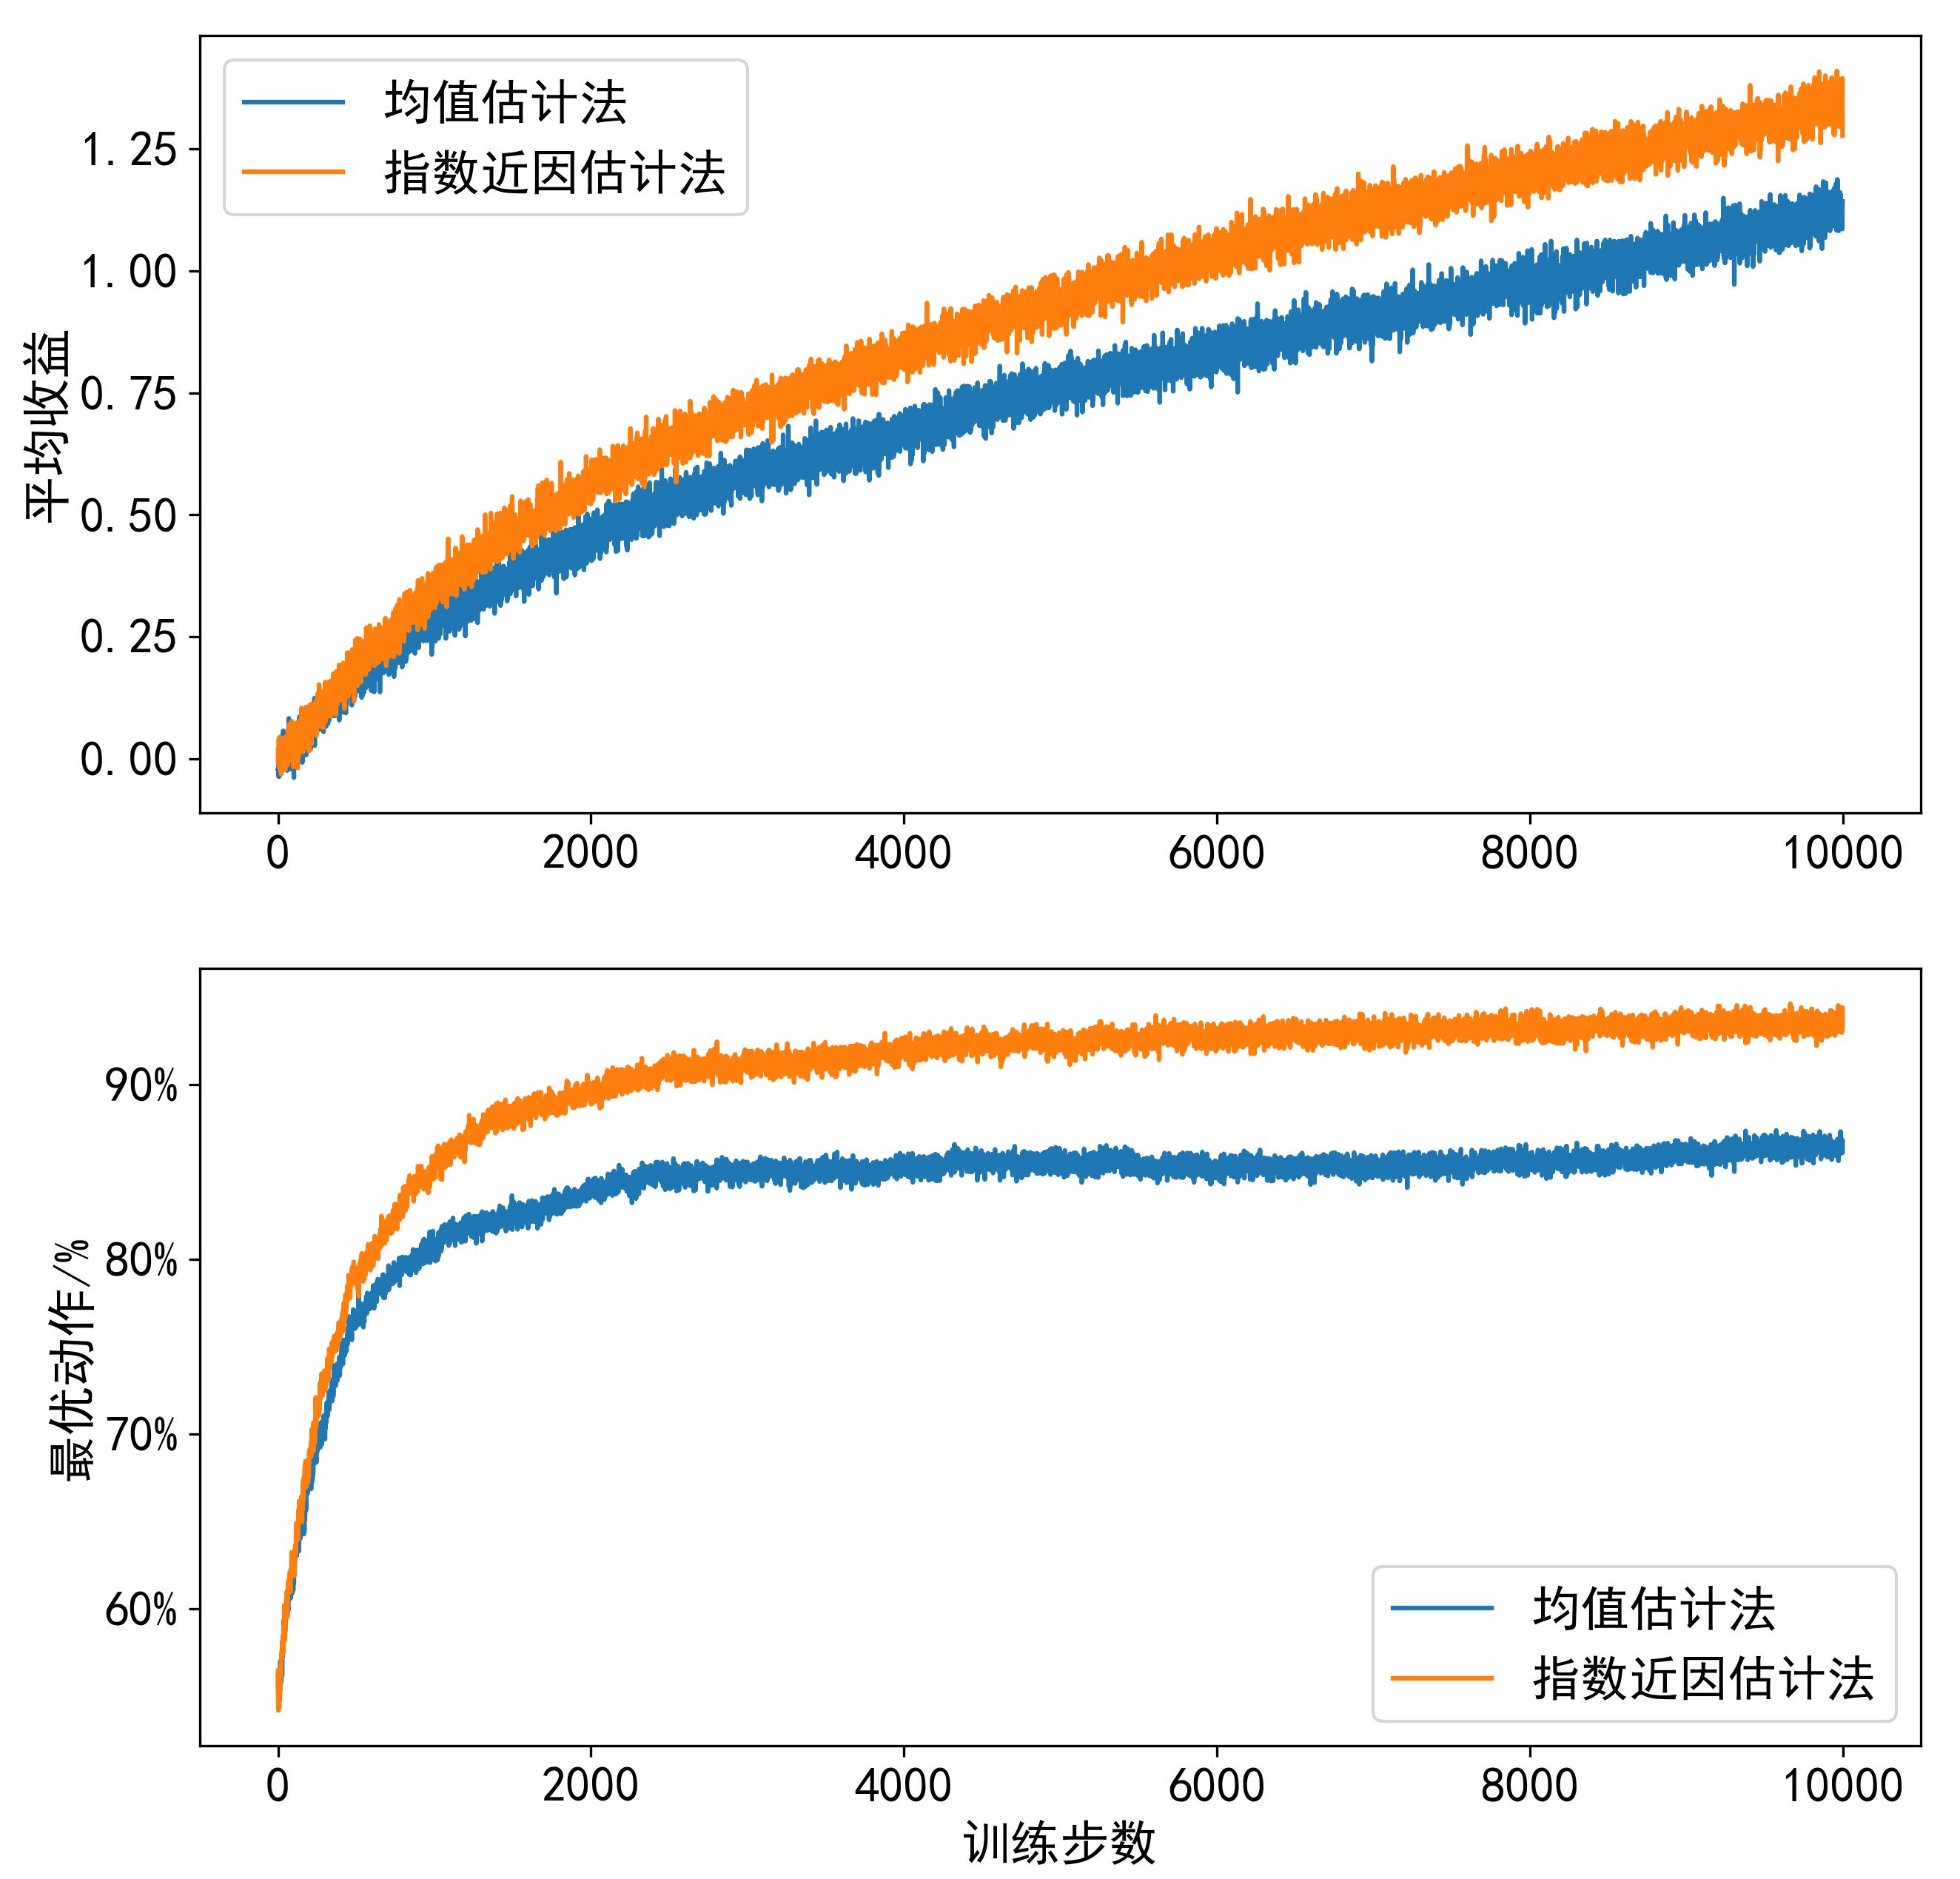
\includegraphics[scale=0.13]{../figures/033/033页练习2.5.png}
    \caption{非稳定问题中均值法与指数近因法的对比}
    \label{fig-averge_recency}
\end{figure}
\section{有限Markov决策}
\subsection{智能体与环境}
有限Markov决策过程(Markov Decision Process, MDP)是指\textbf{智能体(Agent)}与\textbf{环境(Environment)}通过\textbf{动作(Action)}进行交互的过程,
环境返回每个动作的\textbf{收益(Reward)},智能体可以观测到每次动作返回的收益与环境的\textbf{状态(State)},智能体的目标是通过交互从而最大化全局收益,
也就是\textbf{回报(Return)}. 如图\ref{fig-MDP}所示.
\begin{figure}[htbp]
    \centering
    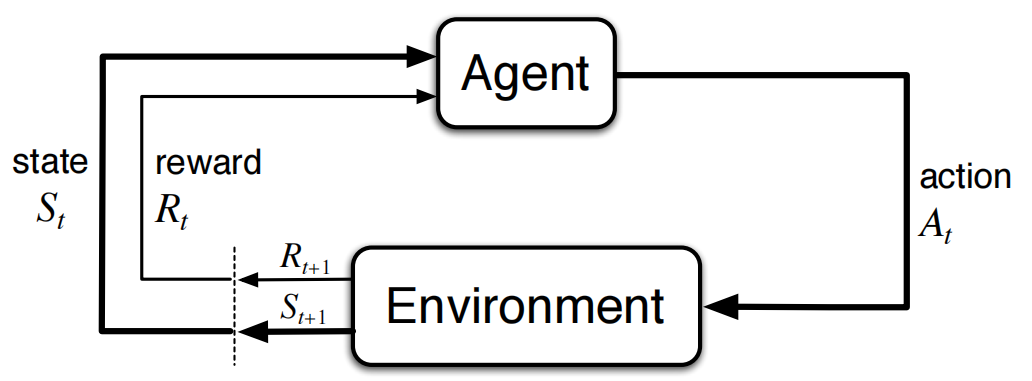
\includegraphics[scale=0.5]{../figures/046页Markov决策中交互图.png}
    \caption{Markov决策交互图}
    \label{fig-MDP}
\end{figure}

在MDP中,状态、收益、动作均为有限集合,分别记为$\S,\R,\A$. 类似游戏中的回合,MDP也有回合的定义称为\textbf{幕(Episode)},任务从开始到结束
称为一幕,将有结束状态的任务称为\textbf{分幕式任务(Episodic task)},否则称为\textbf{持续性任务(Continuning task)}.

将智能体在一幕中观测到的所有状态、动作、收益称为\textbf{轨迹(Trajectory)}:
\begin{equation*}
    S_0,A_0,R_1,S_1,A_1,R_2,S_2,A_2,R_3,\cdots
\end{equation*}
假设状态转移$S_t,R_t$出现的概率仅取决于前一个状态和动作$S_{t-1}, A_{t-1}$,则称符合Markov性质(Markov property),可以表示为下式:
\begin{equation*}
    p(s',r|s,a) := \P\{S_t =s', R_t = r|S_{t-1} = s, A_{t-1} = a\},\quad(s',s\in \S, r\in \R, a\in \A)
\end{equation*}
通过上式可以导出其他类似转移概率
\begin{itemize}
    \item 状态转移概率:$p(s'|s,a) = \sum_{r\in\R}p(s',r|s,a)$;
    \item “状态-动作”收益:$r(s,a) = \E[R_t|S_{t-1} = s, A_{t-1} = a] = \sum_{r\in\R}r\sum_{s'\in\S}p(s',r|s,a)$;
    \item “状态-动作-状态”收益:$r(s,a,s') = \E[R_t|S_{t-1} = s, A_{t-1} = a, S_{t} = s] = \sum_{r\in\R}r\cdot p(r|s,a,s') = \sum_{r\in\R}r\cdot \frac{p(r,s'|s,a)}{p(s'|s,a)}$.
\end{itemize}
回报记为$G_t := R_{t+1}+R_{t+2}+\cdots = \sum_{k=t+1}^\infty R_k$,\textbf{折后回报(Discounted return)}记为
\begin{equation*}
    G_{t}:= R_{t+1}+\gamma R_{t+2}+\gamma^2 R_{t+3} + \cdots = \sum_{k=t+1}^\infty \gamma^{k-t-1}R_k
\end{equation*}
其中$\gamma$称为\textbf{折扣率(Discounted rate)},可以将分幕式任务视为持续性任务统一用上述回报表达式,只需将最终状态后的收益$R$均设置为$0$即可.

可以用递推式表示折扣回报
\begin{align*}
    G_t =&\ R_{t+1} + \gamma R_{t+2}+\gamma^2 R_{t+3}+\cdots\\
    =&\ R_{t+1} + \gamma(R_{t+2}+\gamma R_{t+3}\cdots)\\
    =&\ R_{t+1} + \gamma G_{t+1}
\end{align*}
\subsection{策略与Bellman方程}
\textbf{策略(Policy)}是指智能体基于环境状态$S$相应的动作的函数,具体来讲策略函数$\pi:\S\times \A\to[0,1]$是一个概率密度函数:
\begin{equation*}
    \pi(a|s) = \P_{\pi}[A_t = a| S_t = s]
\end{equation*}

基于给定的策略$\pi$,定义\textbf{策略$\pi$的状态价值函数}$v_\pi(s)$,即在状态$s$下,智能体按照策略$\pi$所能获得的期望回报:
\begin{equation*}
    v_{\pi}(s):= \E_{\pi}[G_t|S_t =s] = \E_{\pi}[R_{t} + \gamma G_{t+1}|S_t = s]
\end{equation*}

类似地,定义\textbf{策略$\pi$的动作价值函数}$q_{\pi}(s,a)$,即在$s$下采取动作$a$后,智能体按照策略$\pi$所能获得的期望回报:
\begin{equation*}
    q_{\pi}(s,a) := \E_{\pi}[G_t|S_t = s, A_t = a] = \E_{\pi}[R_{t+1}+\gamma G_{t+1}|S_t = s, A_t = a]
\end{equation*}

分析$v_{\pi}(s)$的递归关系式,首先注意到$G_{t+1}$的条件概率仅与$S_{t+1}$有关,所以
\begin{align*}
    \E_{\pi}[\gamma G_{t+1}|S_{t}=s] =&\ \gamma\sum_{g}g\cdot p(G_{t+1} = g|s)\\
    \xlongequal{Bayes\text{公式}}&\ \gamma\sum_{g}g\sum_{s'\in \S}p(G_{t+1} = g|S_{t+1}=s',S_t = s)p(s'|s)\\
    \xlongequal{G_{t+1}\text{条件概率仅与}S_{t+1}\text{相关}}&\ \gamma \sum_{s'\in \S}p(s'|s)\sum_{g}g\cdot p(G_{t+1} = g|S_{t+1}=s')\\
    =&\ \gamma\sum_{s'\in \S}p(s'|s)\E[G_{t+1}|S_{t+1} = s']\\
    \xlongequal{Bayes\text{公式}}&\ \gamma\sum_{a}\pi(a|s)\sum_{s',r}p(s',r|s,a)v_{\pi}(s')
\end{align*}
类似地通过Bayes公式可得$\E_{\pi}[R_{t+1}|S_t = s] = \sum_{a}\pi(a|s)\sum_{s',r}p(s',r|s,a)r$,
于是得到\textbf{$v_{\pi}(s)$的Bellman方程}(图\ref{fig-状态价值回溯图}为回溯图,便于形象化理解)\del

{ % 一般将文字环绕部分的图和文字, 用大括号括起来, 避免对文字外的格式发生影响, 有时也不需要自行尝试
\begin{wrapfigure}[3]{r}{.4\linewidth} % 文字环绕行数为13行, 图片靠右 (l为靠左), 图片占0.5的行宽
    \centering
    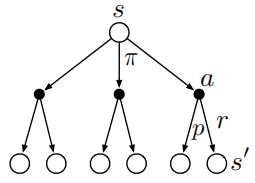
\includegraphics[scale=0.5]{../figures/057页状态价值函数回溯图.png}
    \caption{$v_{\pi}(s)$的回溯图}
    \label{fig-状态价值回溯图}
\end{wrapfigure}
\begin{equation*}
    v_{\pi}(s) = \sum_{a}\pi(a|s)\sum_{s',r}p(s',r|s,a)\big[r + \gamma v_\pi(s')\big]
\end{equation*}
% 这里一定要空一行
}

\noindent 类似地,也有\textbf{$q_{\pi}(s,a)$的Bellman方程}(图\ref{fig-状态动作价值回溯图}为回溯图)\del

{ % 一般将文字环绕部分的图和文字, 用大括号括起来, 避免对文字外的格式发生影响, 有时也不需要自行尝试
\begin{wrapfigure}[13]{r}{.4\linewidth} % 文字环绕行数为13行, 图片靠右 (l为靠左), 图片占0.5的行宽
    \centering
    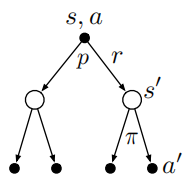
\includegraphics[scale=0.5]{../figures/060页状态价值函数回溯图.png}
    \caption{$q_{\pi}(s,a)$的回溯图}
    \label{fig-状态动作价值回溯图}
\end{wrapfigure}
\begin{equation*}
    q_{\pi}(s,a) = \sum_{r, s',a'}\pi(a'|s')p(s',r|s,a)\big[r + \gamma q_{\pi}(s',a')\big]
\end{equation*}
% 这里一定要空一行
}
\clearpage
而状态价值函数$v_\pi(s)$与$q_\pi(s,a)$满足一下关系式:
\begin{align*}
    v_\pi(s) =&\ \sum_{a}\pi(a|s)q_\pi(s,a)\qquad \text{参考图\ref{fig-状态价值函数由动作价值函数表出}},\\
    q_{\pi}(s,a) = &\ \sum_{s',r}p(s',r|s,a)\big[r+\gamma v_{\pi}(s')\big]\qquad\text{参考图\ref{fig-动作价值函数由状态价值函数表出}}.
\end{align*}

\begin{figure}[htbp]
    \centering
    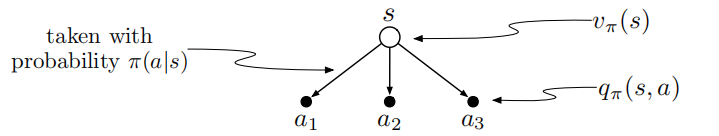
\includegraphics[scale=0.5]{../figures/060页s,(s,a).png}
    \caption{$v_{\pi}(s)$由$q_{\pi}(s,a)$表出}
    \label{fig-状态价值函数由动作价值函数表出}
\end{figure}

\begin{figure}[htbp]
    \centering
    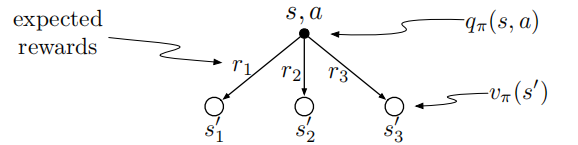
\includegraphics[scale=0.5]{../figures/060页(s,a),s.png}
    \caption{$q_{\pi}(s,a)$由$v_{\pi}(s')$表出}
    \label{fig-动作价值函数由状态价值函数表出}
\end{figure}
\subsection{最优策略与最优价值函数}
定义\textbf{最优状态价值函数}$v_*$满足$\forall s\in \S$有$v_*(s) = \max_{\pi}v_{\pi}(s)$成立;
类似地,定义\textbf{最优动作价值函数}满足$\forall s\in \S, a\in\A$有$q_*(s,a) = \max_{\pi}q_*(s,a)$成立.
两者的关系为
\begin{equation*}
    q_*(s,a) = \E[R_{t+1}+\gamma v_*(S_{t+1})|S_t =s, A_t = a] = \sum_{s', r}p(s',r|s,a)\big[r+\gamma v_*(s')\big].
\end{equation*}

通过修改Bellman方程,只需将$\sum_{a}\pi(a|s)$改为$\max_{a}$,$v_\pi(s)$改为$v_*(s)$,
$q_{\pi}(s,a)$改为$q_*(s,a)$即可得到\textbf{Bellman}最优方程(对应的回溯图如图\ref{fig-状态与动作最优价值函数回溯图}所示):
\begin{align*}
    v_*(s) =&\ \max_{a}\sum_{s',r}p(s',r|s,a)\big[r+\gamma v_*(s')\big],\\
    q_*(s,a) =&\ \sum_{s',r}p(s',r|s,a)\big[r+\gamma\max_{a'}q_*(s',a')\big].
\end{align*}
\begin{figure}[htbp]
    \centering
    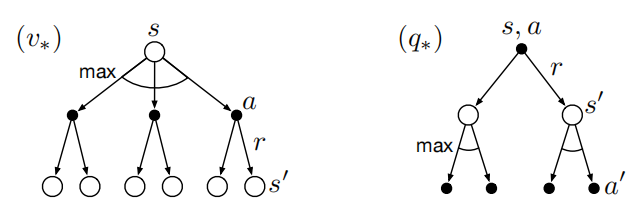
\includegraphics[scale=0.5]{../figures/062页状态与动作最优价值函数回溯图.png}
    \caption{$v_*(s)$与$q_*(s,a)$的回溯图}
    \label{fig-状态与动作最优价值函数回溯图}
\end{figure}
下面将用已有的轨迹估计$v_*(s)$和$q_*(s,a)$,根据使用轨迹的不同长度和对Markov性质的已知情况分为以下三种策略:

\begin{enumerate}
    \item 动态规划(DP):环境是完备的,智能体对Markov性质完全了解,$p(s',r|s,a)$分布已知.
    \item 蒙特卡洛方法(MC):环境是未知的,只能通过交互获得分布的近似,通过整个轨迹反向估计$G_t$.
    \item 时序差分方法(TD):环境是未知的,只能通过交互获得分布的近似,仅通过两步之间的结果估计$G_t$.
\end{enumerate}

\section{动态规划}
动态规划(Dynamic Programming, DP)可以在给定Markov决策过程的完备环境模型下,计算最优策略.

\subsection{策略评估}
对于给定的策略$\pi(a|s)$,DP方法首先需要通过迭代的方式得到状态价值函数,迭代式如下所示
\begin{equation*}
    v_{k+1}(s) = \sum_{a}\pi(a|s)\sum_{s',r}p(s',r|s,a)\big[r+\gamma v_k(s')\big]
\end{equation*}
初始值$v_0(s) = 0,\quad (\forall s\in \S)$.

\subsection{策略改进}
\begin{theorem}[策略改进定理]
    设$\pi,\pi'$为任意两个确定的策略,$\forall s\in \S$,有
    \begin{equation*}
        q_{\pi}(s,\pi'(s)) \geq v_\pi(s)
    \end{equation*}
    则称策略$\pi'$和$\pi$一样好或更好,并且$v_{\pi'}(s)\geq v_{\pi}(s)$. 也就是说如果$\pi'(s) = a$且$q_{\pi}(s,a) \geq v_{\pi}(s)$,
    除去$s$的其他状态下$\pi=\pi'$,那么改进后的策略$\pi'$一定比$\pi$更优.
\end{theorem}

策略改进定理本质就是贪心的结果,这说明根据策略评估结果,只需贪心选择状态价值更高的策略更新已有的策略即可得到更优的策略,贪心策略$\pi'$满足
\begin{equation*}
    \pi'(s):= \argmax_{a}q_{\pi}(s, a) = \argmax_{a}\sum_{s',r}p(s',r|s,a)\big[r+\gamma v_{\pi}(s')\big].
\end{equation*}
不难发现这和最优状态价值函数的Bellman方程基本一致,只需将$v_{\pi}$改为$v_{\pi'}$即可,说明通过不断使用贪心策略进行改进,一定将状态价值函数逼近最优状态价值函数,
从而得到最优策略.

总的来说,动态规划有两种迭代方案:

1. \textbf{策略迭代}:先进行评估再进行改进即可:
\begin{equation*}
    \pi_0\xrightarrow{E}v_{\pi_0}\xrightarrow{I}\pi_1\xrightarrow{E}v_{\pi_1}\xrightarrow{I}\pi_2\xrightarrow{E}\cdots\xrightarrow{I}\pi_*\xrightarrow{E}v_*,
\end{equation*}
其中$\xrightarrow{E}$表示策略评估,$\xrightarrow{I}$表示策略改进,直到策略$\pi_k = \pi_{k+1}$时停止迭代.

2. \textbf{价值迭代}:直接使用最优状态价值函数进行迭代
\begin{equation*}
    v_{k+1}(s) = \max_a\sum_{s',r}p(s',r|s,a)\big[r+\gamma v_k(s')\big]
\end{equation*}
最后确定最优策略$\pi_*$的近似策略$\pi$:
\begin{equation*}
    \pi(s) = \argmax_{a}\sum_{s',r}p(s',r|s,a)\big[r+\gamma v(s')\big]
\end{equation*}
\section{蒙特卡洛方法}
蒙特卡洛方法(Monte Carlo, MC),MC仅需智能体的经验,无需完备的环境知识,可以通过经验中进行学习,
思路是通过一幕的平均样本回报来估计价值函数.

\subsection{蒙特卡洛预测}
由折扣回报的定义可知$G_{t} = R_{t+1} + \gamma G_{t+1}$,对于已生成的一幕序列
\begin{equation*}
    S_0,A_0,R_1,S_1,A_1,\cdots, S_{T-1}, A_{T-1},R_T
\end{equation*}
可以倒序计算每个时刻的$G_{t}$,初始化$G_{T} = 0$,然后倒序依次计算
\begin{equation*}
    G_{t} = R_{t+1}+\gamma G_{t+1},\ (t=T-1,T-2,\cdots,0)   
\end{equation*}
然后将$G_t$用于更新$S_t$处的状态$s_t$对应的价值函数$v_{\pi}(s_t) = \E(G_t|S_t = s_t)$,\add
可以用递推式进行更新$v_{\pi}(s_t) \leftarrow v_{\pi}(s_t) + \frac{1}{n}(G_t - v_{\pi}(s_t))$\add ,
其中$n$为$s_t$在之前幕中出现的总次数,也就是求$n$个状态价值$G_t$的均值作为$v_{\pi}(s_t)$的估计.

在一幕中,某一状态$s\in\S$可能被多次访问到,如果只对第一次出现的$s$的状态价值函数进行更新,称为\textbf{首次访问型MC预测算法(First visit MC)};
如果对每次出现的$s$的状态价值均进行更新,称为\textbf{每次访问型MC预测算法(Every visit MC)}.

类似地可以用蒙特卡洛方法对动作价值函数$q_{\pi}(s,a)$进行预测,方法与状态价值函数完全相同. 由于部分动作价值函数可能永远无法访问到,
所以引入两种解决方法:
\begin{enumerate}
    \item 试探性出发假设:每一幕的出发状态是选定的“状态-动作”二元组,从而保证每个$(s,a)$组合可以遍历到.
    \item 每个状态下做出策略时,所有动作都有非零的概率被选中(也就是$\varepsilon$-软性策略).
\end{enumerate}
\subsection{蒙特卡洛控制}
基本思想与DP中使用的广义策略迭代(Generalized Policy Iteration, GPI)相同,考虑同时维护一个近似的策略
和近似的价值函数,近似价值函数通过迭代逼近当前策略的最优价值函数,而当前策略会根据价值函数不断调优,彼此为对方设定优化目标,
从而使得策略和价值函数同时趋向最优解,如图\ref{fig-广义策略迭代与蒙特卡洛控制}所示.
\begin{figure}[htbp]
    \centering
    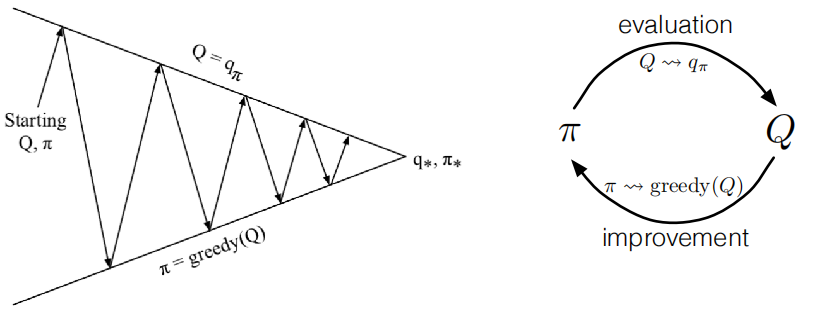
\includegraphics[scale=0.6]{../figures/095页广义策略迭代与蒙特卡洛控制.png}
    \caption{广义策略迭代与蒙特卡洛控制}
    \label{fig-广义策略迭代与蒙特卡洛控制}
\end{figure}

策略改进方法仍与DP相同,贪心地选取$\pi'(s) = \argmax_{a}q_{\pi}(s,a)$,即可保证$\pi'$至少不必$\pi$更坏.

最简单的蒙特卡洛控制是基于试探性出发的,在每次更新完成$q(s_t, a_t)$后,更新策略$\pi(s_t)\rightarrow \argmax_{a}q(s_t, a)$.

第二种蒙特卡洛控制是基于$\varepsilon$-软性策略,假设状态$s\in\S$下的动作集合记为$\A(s)$,则每一个动作
均至少有$\frac{\varepsilon}{|\A(s)|}$的概率被选中,也就是更新后的策略为
\begin{equation*}
    \pi(a|s) = \begin{cases}
        \varepsilon / |\A(s)| + 1 - \varepsilon,&\quad a = \argmax_{a\in\A}q(s,a),\\
        \varepsilon / |\A(s)|,&\quad \text{否则}.
    \end{cases}
\end{equation*}

上述方法称为\textbf{同轨策略(on-policy)},也就是用于生成采样数据的策略与实际不断改进的策略相同;
还有一种方法称为\textbf{离轨策略(off-policy)},也就是用于生成采样数据的策略与实际改进的策略不同.

\subsection{基于重要度采样的离轨策略}
将离轨策略中用于生成样本的策略记为$b$,一般要求策略$b$能够覆盖当前更新的$\pi$,也就是指$\pi(a|s) > 0$时
有$b(a|s) > 0$,由于策略$b$与策略$\pi$生成同一个轨迹具有差异,定义\textbf{重要度采样比}来衡量二者的差异大小,
状态-动作轨迹$A_t,S_{t+1},A_{t+1},\cdots, S_{T}$在策略$\pi$下发生的概率为
\begin{align*}
    &\ \P\{A_t,S_{t+1},A_{t+1},\cdots, S_{T}|S_t, A_{t:T-1}\sim \pi\}\\
    =&\ \pi(A_t|S_t)p(S_{t+1}|S_t,A_t)\pi(A_{t+1}|S_{t+1})\cdots p(S_T|S_{T-1},A_{T-1})\\
    =&\ \prod_{k=t}^{T-1}\pi(A_k|S_k)p(S_{k+1}|S_k,A_k)
\end{align*}
于是$\pi,b$在$t:T-1$段上的重要度采样比为
\begin{equation*}
    \rho_{t:T-1} = \frac{\prod_{k=t}^{T-1}\pi(A_k|S_k)p(S_{k+1}|S_k,A_k)}{\prod_{k=t}^{T-1}b(A_k|S_k)p(S_{k+1}|S_k,A_k)} = 
    \prod_{k=t}^{T-1}\frac{\pi(A_k|S_k)}{b(A_k|S_k)}.
\end{equation*}
这里给出两种根据重要度采样比调整回报加权平均的方法:
\begin{align*}
    \text{普通重要度采样: }v(s) =&\ \frac{\sum_{t\in\mathcal{T}(s)}\rho_{t:T(t)-1}G_t}{|\mathcal{T}(s)|},\\
    \text{加权重要度采样: }v(s) =&\ \frac{\sum_{t\in\mathcal{T}(s)}\rho_{t:T(t)-1}G_t}{\sum_{t\in\mathcal{T}(s)}\rho_{t:T(t)-1}}.
\end{align*}
其中$\mathcal{T}(s)$表示所有访问过状态$s$的时刻集合,将所有幕连续地编号,并用$T(t)$表示$t$时刻后的首次中止时刻. 
上述两种加权方式中,普通重要度采样是无偏的但是方差无界的,而加权重要度采样是有偏但是方差有界的,一般使用加权重要度采样.

类似地,我们也有\textbf{增量式更新加权采样的方法},假设
\begin{equation*}
    v_n = \frac{\sum_{k=1}^{n-1}w_kG_k}{\sum_{k=1}^{n-1}w_k} =\frac{\sum_{k=1}^{n-1}w_kG_k}{c_{n-1}}
\end{equation*}
则增量式更新方法为
\begin{equation*}
    v_{n+1} = v_n + \frac{w_n}{c_n}(G_n - v_n),\quad c_{n+1} = \sum_{k=1}^{n+1}w_k = c_n + w_{n+1}
\end{equation*}
\section{时序差分学习}
时序差分学习(Temporal-Difference Learning, TD)
\end{document}
